% !TEX root = main.tex

\section{对偶理论}
\subsection{拉格朗日对偶}
\begin{definition}[拉格朗日函数(Lagrangian function)]
$f_i(\vx)$和$h_j(\vx)$含义同\ref{sub:convex_opt_def}节,前者不等式约束($\leq 0$),后者等式约束。
\[\begin{aligned}
    L(\vx,\vlambda,\vv)&=f_0(\vx)+\sum_{i=1}^m\lambda_if_i(\vx)+\sum_{i=1}^pv_ih_i(\vx)\\
    &=f_0(\vx) + \vlambda^\T \vf(\vx)+\vv^\T \vh(\vx),\;\dom L=\sD\times \rr^m\times \rr^p
\end{aligned}\]
\end{definition}

\begin{definition}[拉格朗日乘子(multiplier)]
    对偶变量即拉格朗日乘子
\begin{itemize}
\item 原变量(primal variable):$\vx$
\item 对偶变量(dual variable):$\vlambda=\bmat{\lambda_1 & \cdots & \lambda_m}^\T,\;\vv=\bmat{v_1 & \cdots & v_p}^\T$
\end{itemize}
\end{definition}

\begin{definition}[拉格朗日对偶函数]
\[\begin{aligned}
    g(\vlambda,\vv)&=\inf_{\vx\in\sD} L(\vx,\vlambda,\vv)\\
    &=\inf_{\vx\in\sD}\lrp{f_0(\vx)+\sum_{i=1}^m\lambda_if_i(\vx)+\sum_{i=1}^pv_ih_i(\vx)}
\end{aligned}\]
注意\textcolor{red}{遍历域是$\sD=\bigcap_{i=0}^m\dom f_i\cap\bigcap_{i=1}^p\dom h_i$},而不是可行解集$\sX$\\
如果约束$f$和$h$为标量,那么$v$和$\lambda$也对应改为标量;如果有多个向量约束,可对应添加对偶变量
\end{definition}

有以下两点性质:
\begin{itemize}
    \item $g(\vlambda,\vv)$一定是关于$\vlambda$和$\vv$的凹函数(关于$\vlambda$和$\vv$的仿射函数,注意$\vx$为常数)
    \item $\forall\vlambda\succeq \vzero,\forall \vv:\;g(\vlambda,\vv)\leq p^\star$
\end{itemize}

\begin{definition}[对偶(dual)问题]
    \begin{maxi*}
        {}{g(\vlambda,\vv)}{}{}
        \addConstraint{\vlambda}{\succeq \vzero}
    \end{maxi*}
    其最优解记为$d^\star$,则$d^\star\leq p^\star$,即给出了原问题(primal)的一个\textbf{最优下界}
\end{definition}
\begin{analysis}
    记$\vx^\star$为原问题最优解,由优化问题定义有
    \[\sum_{i=1}^m\lambda_i f_0(\vx^\star)+\sum_{i=1}^p v_i h_i(\vx^\star)\leq 0\]
    又$p^\star=f_0(\vx^\star)$为原问题最优解,将$\vx^\star$代入Lagrange函数中
    \[L(\vx^\star,\vlambda,\vv)=f_0(\vx^\star)+\lrp{\sum_{i=1}^m\lambda_i f_0(\vx^\star)+\sum_{i=1}^p v_i h_i(\vx^\star)}\leq p^\star\]
    进而推出
    \[g(\vlambda,\vv)=\inf_{\vx\in\sD} L(\vx,\vlambda,\vv)\leq L(\vx^\star,\vlambda,\vv)\leq p^\star\]
\end{analysis}

\begin{example}[最小二乘]
\begin{mini*}
    {}{\norm{\vx}_2=\vx^\T \vx}{}{}
    \addConstraint{A\vx}{=\vb}
\end{mini*}
\end{example}
\begin{analysis}
\[\begin{aligned}
    L(\vx,\vv)&=\vx^\T \vx+\vv^\T(A\vx-\vb)\\
    g(\vv)&=\inf_{\vx\in\sD} L(\vx,\vv)\\
    &=\inf_{\vx\in\sD} \lrp{\vx^\T \vx+\vv^\T A \vx-\vv^\T \vb}\qquad\mbox{求最小值相当于求导/求梯度代入}\\
    &=\lrp{-\frac{A^\T \vv}{2}}^\T\lrp{-\frac{A^\T \vv}{2}}+\vv^\T A\lrp{-\frac{A^\T \vv}{2}}-\vv^\T \vb\\
    &=-\frac{1}{4}\vv^\T A A^\T \vv-\vb^\T \vv
\end{aligned}\]
\par 补充求梯度:$\nabla_\vx L(\vx,\vv)=2\vx+(\vv^\T A)^\T=0\implies \vx=-\frac{A^\T \vv}{2}$
\par 因而得到对偶问题
\[\max_\vv\lrp{-\frac{1}{4}\vv^\T A A^\T \vv-\vb^\T \vv}\]
\end{analysis}

\begin{example}[标准线性规划]
\begin{mini*}
    {}{\vc^\T \vx}{}{}
    \addConstraint{A\vx}{=\vb}
    \addConstraint{\vx}{\succeq \vzero}
\end{mini*}
\end{example}
\begin{analysis}
    $1\degree$ \textcolor{red}{注意$\vlambda$前面符号},要化为一般形式
    \[L(\vx,\vlambda,\vv)=\vc^\T \vx-\vlambda^\T \vx+\vv^\T(A\vx-\vb)\]
    \[\begin{aligned}
        g(\vlambda,\vv)&=\inf_\vx L(\vx,\vlambda,\vv)\\
        &=\inf_\vx\lrp{(\vc-\vlambda+A^\T \vv)^\T \vx-\vv^\T \vb}\\
        \quad\mbox{一次式应直接分拆变量和常量,由于$\vx$可以任取,故会到负无穷}
        &=\begin{cases}-\infty & \vc-\vlambda+A^\T \vv\ne 0\\
        -\vv^\T \vb & \vc-\vlambda+A^\T \vv=0\end{cases}
    \end{aligned}\]
    由于要极大,故不考虑负无穷部分,得到对偶问题如下
    \begin{maxi*}
        {\vlambda,\vv}{-\vv^\T \vb}{}{}
        \addConstraint{\vc-\vlambda+A^\T \vv}{=0}
        \addConstraint{\vlambda}{\succeq \vzero}
    \end{maxi*}
    $2\degree$ 考虑对偶问题的对偶,先将对偶问题变为极小化问题
    \begin{mini*}
        {}{\vb^\T \vv}{}{}
        \addConstraint{A^\T \vv+\vc}{\succeq \vzero}
    \end{mini*}
    \[L(\vv,\vlambda)=\vb^\T \vv-\vlambda^\T(A^\T \vv+\vc)\]
    \[\begin{aligned}
        g(\vlambda)&=\inf_\vv L(\vv,\vlambda)\\
        &=\inf_\vv\lrp{(\vb-A\vlambda)^\T \vv-\vlambda^\T \vc}\\
        &=\begin{cases}
            -\vlambda^\T \vc & \vb-A\vlambda =0\\
            -\infty & \vb-A\vlambda\ne 0
        \end{cases}
    \end{aligned}\]
    得到新的对偶问题
    \begin{maxi*}
        {}{-\vlambda^\T \vc}{}{}
        \addConstraint{\vb-A\vlambda}{=0}
        \addConstraint{\vlambda}{\succeq 0}
    \end{maxi*}
    会发现,对偶的对偶不一定回去,线性规划才满足
\end{analysis}
% 对偶支撑向量机(SVM) 升变量维度,降约束维度

\begin{example}[二路分划(two-way partitioning)]
    非凸问题,考虑可行解集有$2^n$个离散点,将$\{1,\ldots,n\}$分划到两个集合中,$W_{ij}$是将$i,j$指派到同一个集合的开销,$-W_{ij}$是将$i,j$指派到不同集合的开销
\begin{mini*}
    {}{\vx^\T W\vx}{}{}
    \addConstraint{x_i}{=\pm 1,}{\quad i=1,\ldots,n}
\end{mini*}
\end{example}
\begin{analysis}
    变为平方等式约束
    \[\begin{aligned}
        L(\vx,\vv)&=\vx^\T W\vx+\sum_{i=1}^n v_i(x_i^2-1)\\
        g(\vv)&=\inf_\vx L(\vx,\vv)\\
        &=\inf_\vx \lrp{\vx^\T W\vx+\sum_{i=1}^n v_ix_i^2-\sum_{i=1}^n v_i}\qquad\mbox{二次项放对角线}\\
        &=\inf_\vx \lrp{\vx^\T\lrp{W+\opdiag \vv}\vx-\vone^\T \vv}\\
        &=\begin{cases}-\vone^\T \vv & W+\opdiag(\vv)\succeq \vzero\\-\infty&\text{otherwise}\end{cases}
    \end{aligned}\]
    其中
    \[\opdiag\vv=\bmat{v_1 & \cdots & 0\\\vdots & \ddots & \vdots\\0 & \cdots & v_n}\]
    得到对偶问题如下
    \begin{maxi*}
        {\vv}{-\vone^\T \vv}{}{}
        \addConstraint{W+\opdiag(\vv)}{\succeq \vzero}
    \end{maxi*}
\end{analysis}

\begin{example}[共轭函数]
\begin{mini*}
    {}{f_0(\vx)}{}{}
    \addConstraint{A\vx}{\leq \vb}
    \addConstraint{C\vx}{=\vd}
\end{mini*}
\end{example}
\begin{analysis}
\[\begin{aligned}
    L(\vx,\vlambda,\vv)&=f_0(\vx)+\vlambda^\T(A\vx-\vb)+\vv^\T(C\vx-\vd)\\
    &=f_0(\vx)+(A^\T\vlambda+C^\T \vv)^\T \vx-\vlambda^\T \vb-\vv^\T \vd\\
    g(\vlambda,\vv)&=\inf_\vx \lrp{f_0(\vx)+(A^\T\vlambda+C^\T \vv)^\T \vx-\vlambda^\T \vb-\vv^\T \vd}\\
    &=-\sup_\vx\lrp{-(A^\T\vlambda+C^\T \vv)^\T \vx-f_0(\vx)}-\vlambda^\T \vb-\vv^\T \vd\\
    &=-f_0^\star(-(A^\T\vlambda+C^\T \vv))-\vlambda^\T \vb-\vv^\T \vd
\end{aligned}\]
\end{analysis}

\subsection{强弱对偶}
\begin{definition}[对偶间隙(duality gap)]
    $p^\star-d^\star\geq 0$
\begin{itemize}
    \item 弱对偶:严格大于0
    \item 强对偶:对偶间隙为0
\end{itemize}
\end{definition}

\begin{enumerate}
    \item 对于非凸问题,\textbf{通常}$p^\star\ne d^\star$
    \item 对于凸问题,若满足Slater条件,则$p^\star=d^\star$
\end{enumerate}

\begin{definition}[相对内点(relative interior)]
    存在一个邻域所有的点都落在集合内,即多元微积分中内点的概念。
    而相对内点则是考虑仿射包$\opaff \sD$的情况
    \[\oprelint \sD=\{\vx\in \sD\mid B(\vx,r)\cap\opaff \sD\subset \sD,\exists r>0\}\]
\end{definition}

\begin{theorem}[Slater条件]
强对偶对于下列凸问题成立
\begin{mini*}
    {}{f_0(\vx)}{}{}
    \addConstraint{f_i(\vx)}{\leq 0}{,\quad i=1,\ldots,m}
    \addConstraint{A\vx}{=\vb}
\end{mini*}
若它严格可行,即
\[\exists \vx\in\oprelint \sD,\;\text{s.t.}\;f_i(\vx)<0,\;i=1,\ldots,m,\;A\vx=\vb\]
\end{theorem}

\begin{example}
    二次规划(QP)
    \begin{mini*}
        {}{\vx^\T \vx}{}{}
        \addConstraint{A\vx}{=\vb}
    \end{mini*}
    Slater条件$\{\vx\mid A\vx=\vb\}$非空
\end{example}
\begin{example}[二次约束二次规划(QCQP)]
    \begin{mini*}
        {}{\frac{1}{2}\vx^\T P_0 \vx+\vq_0^\T+r_0}{}{}
        \addConstraint{\frac{1}{2}\vx^\T P_i \vx+\vq_i^\T \vx+r_i}{\leq 0}{,\quad i=1,\ldots,m}
    \end{mini*}
    $P_0,\ldots,P_m$半正定
\end{example}

凸问题+Slater条件$\implies p^\star=d^\star$,但有可能不满足Slater条件也依然强对偶,如下面的例子。
\begin{example}
\begin{mini*}
    {}{x,\;x\in\rr}{}{}
    \addConstraint{x}{\leq 0}
    \addConstraint{-x}{\leq 0}
\end{mini*}
\end{example}
\begin{analysis}
    \[\begin{aligned}
        L(x,\lambda_1,\lambda_2)&=x+\lambda_1 x-\lambda_2 x=(1+\lambda_1-\lambda_2)x\\
        g(\lambda_1,\lambda_2)&=\inf_{x\in\rr}(1+\lambda_1-\lambda_2)x=
    \begin{cases}0& 1+\lambda_1-\lambda_2=0\\ -\infty &\text{otherwise}\end{cases}
    \end{aligned}\]
    \par 得到对偶问题
    \begin{maxi*}
        {\lambda_1,\lambda_2}{0}{}{}
        \addConstraint{1+\lambda_1-\lambda_2}{=0}
    \end{maxi*}
    \par 可以推出$p^\star=d^\star=0$
\end{analysis}

\begin{example}[置信域问题]
\begin{mini*}
    {}{\vx^\T A\vx+\vb^\T \vx}{}{}
    \addConstraint{\vx^\T \vx}{\leq 1}
    \addConstraint{A}{\nsucceq 0}
\end{mini*}
依然可以得到$p^\star=d^\star$
\end{example}

\subsection{对偶问题的几种解释}
\subsubsection{几何解释}
考虑问题只有一个约束$f_1(\vx)\leq 0$,记$\sG=\{(f_1(\vx),f_0(\vx))\mid \vx\in\sD\}$,则原问题最优解
\[p^\star=\inf\{t\mid(u,t)\in \sG,u\leq 0\}\]
对偶函数如下,相当于给定斜率,在$\sG$内找点使$t+\lambda u$最小
\[g(\lambda)=\inf\{t+\lambda u\mid(u,t)\in \sG\}\]
对偶问题为
\begin{maxi*}
    {}{g(\lambda)}{}{}
    \addConstraint{\lambda}{\geq 0}
\end{maxi*}
左图即在$u\leq 0$的部分找$t$的最小值,得到$p^\star$;右图得到对偶函数的最大值$d^\star$
\begin{figure}[H]
    \centering
    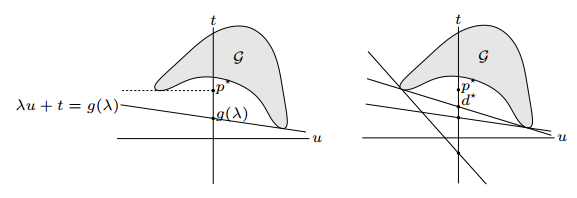
\includegraphics[width=0.5\linewidth]{fig/dual-geo.PNG}
\end{figure}
注意问题必须要有可行解

\subsubsection{经济学解释}
满足原材料约束下,利润最多,价格$\lambda_i\geq 0$,极小化成本
\[g(\vlambda)=\inf_\vx \lrp{f_0(\vx)+\lambda_1 f_1(\vx)+\cdots+\lambda_m f_m(\vx)}=\inf_\vx L(\vx,\vlambda)\]
则$g(\vlambda)$为对偶函数,市场$p^\star$损失最小($g(\vlambda)\leq \vp^\star$)
\[d^\star=\sup_{\vlambda}g(\vlambda)\]
市场平衡点,均衡市场$p^\star=d^\star$,最优/影子价格$\vlambda^\star$

\subsubsection{多目标优化解释}
\[\begin{cases}
    \min f_0(\vx) & 1\\
    \min f_1(\vx) & \lambda_1\\
    \vdots & \vdots\\
    \min f_m(\vx) & \lambda_m
\end{cases}\]
\[\min_\vx \lrp{f_0(\vx)+\lambda_1 f_1(\vx)+\cdots+\lambda_m f_m(\vx)}\]

\subsubsection{鞍点(saddle point)解释}
考虑函数$f(\vw,\vz),\vw\in \sW,\vz\in \sZ$
极小极大不等式
\[\sup_{\vz\in \sZ}\inf_{\vw\in \sW} f(\vw,\vz)\leq \inf_{\vw\in \sW}\sup_{\vz\in \sZ}f(\vw,\vz)\]
\begin{definition}[鞍点]
若有$(\tilde{\vw},\tilde{\vz})$使得
\[\begin{aligned}
    (\tilde{\vw},\tilde{\vz})&=\argmax_{\vz\in \sZ}\min_{\vw\in \sW} f(\vw,\vz)\\
    (\tilde{\vw},\tilde{\vz})&=\argmin_{\vw\in \sW}\max_{\vz\in \sZ} f(\vw,\vz)
\end{aligned}\]
则$(\tilde{\vw},\tilde{\vz})$为鞍点,即下面不等式成立
\[\forall \vz\in \sZ,\vw\in \sW:\;f(\tilde{\vw},\vz)\leq f(\tilde{\vw},\tilde{\vz})\leq f(\vw,\tilde{\vz})\]
相当于从一个方向望过去是最小,从另一个方向望过去是最大
\end{definition}

\[\begin{aligned}
    \qquad & L(\vx,\vlambda)=f_0(\vx)+\sum_{i=1}^m\lambda_i f_i(\vx)\\
    \implies& \sup_{\vlambda\succeq \vzero}L(\vx,\vlambda)=\sup_{\vlambda\succeq \vzero}\lrb{f_0(\vx)+\sum_{i=1}^m\lambda_if_i(\vx)}=
    \begin{cases}f_0(\vx)&f_i(\vx)\leq 0,i=1,\ldots,m\\+\infty&\text{otherwise}\end{cases}\\
    \implies& p^\star =\inf_\vx\lrb{f_0(\vx)\mid f_i(\vx)\leq 0,i=1,\ldots,m}=\inf_\vx\sup_{\vlambda\succeq \vzero}L(\vx,\vlambda)
\end{aligned}\]
由极小极大不等式可得
\[d^\star=\sup_{\vlambda\succeq 0}\inf_\vx L(\vx,\vlambda)\leq\inf_\vx\sup_{\vlambda\succeq 0}L(\vx,\vlambda)=p^\star\]

鞍点在无约束优化问题中是很糟糕的点(所有方向上梯度为0),但是有约束优化问题中则是非常好的点。

\begin{theorem}
    $(\tilde{\vx},\tilde{\vlambda})$为拉格朗日函数鞍点$\iff p^\star=d^\star$,且$(\tilde{\vx},\tilde{\vlambda})$为原对偶问题的最优解
    \[\begin{cases}
        \disp\tilde{\vx}=\arginf_\vx\sup_{\vlambda\succeq \vzero}L(\vx,\vlambda)\\
        \disp\tilde{\vlambda}=\argmax_{\vlambda\succeq \vzero}\inf_\vx L(\vx,\vlambda)
    \end{cases}\]
\end{theorem}
\begin{analysis}
    右推左,$(\tilde{\vx},\tilde{\vlambda})$为原对偶问题可行解
    \[f_i(\tilde{\vx})\leq 0,i=1,\ldots,m,\tilde{\vlambda}\succeq \vzero\]
    因$p^\star=d^\star$,有
    \[\begin{aligned}
        f_0(\tilde{\vx})&=g(\tilde{\vlambda})\\
        &=\inf_\vx\lrb{f_0(\vx)+\sum_{i=1}^m\tilde{\lambda}_i f_i(\vx)}\qquad\mbox{最小值必然比其他值都小}\\
        &\leq f_0(\tilde{\vx})+\sum_{i=1}^m\tilde{\lambda}_i f_i(\tilde{\vx})\qquad\mbox{约束条件}\\
        &\leq f_0(\tilde{\vx})
    \end{aligned}\]
    进而不等号都得为等号,还可得到
    \begin{enumerate}
        \item $\disp \inf_\vx L(\vx,\tilde{\vlambda})=L(\tilde{\vx},\tilde{\vlambda})$(由第一条不等式)
        \item $\disp f_0(\tilde{\vx})=\sup_{\vlambda\succeq \vzero}\lrb{f_0(\tilde{\vx})+\sum_{i=1}^m\lambda_i f_i(\tilde{\vx})}=\sup_{\vlambda\succeq \vzero}L(\tilde{\vx},\vlambda)=L(\tilde{\vx},\tilde{\vlambda})$(由第二条不等式)
    \end{enumerate}
    故右推左成立
\end{analysis}

\subsection{一般优化问题的对偶理论}
\begin{mini*}
    {}{f_0(\vx)}{}{}
    \addConstraint{f_i(\vx)}{\leq 0}{,\quad i=1,\ldots,m}
    \addConstraint{h_i(\vx)}{=0}{,\quad i=1,\ldots,p}
\end{mini*}
不一定是凸问题,但$p^\star=d^\star$,最优解满足什么条件?

设其对偶问题为下式
\begin{maxi*}
    {}{g(\vlambda,\vv)}{}{}
    \addConstraint{\vlambda}{\succeq \vzero}
\end{maxi*}
\begin{analysis}
    设$(\vx^\star,\vlambda^\star,\vv^\star)$为原对偶最优解,则$(\vx^\star,\vlambda^\star,\vv^\star)$为原对偶可行解
    \[f_i(\vx^\star)\leq 0,i=1,\ldots,m,\quad h_i(\vx^\star)=0,i=1,\ldots,p,\quad\vlambda^\star\geq 0\]
    \[\begin{aligned}
        \vp^\star=\vd^\star\implies f_0(\vx^\star)&=g(\vlambda^\star,\vv^\star)\\
        &=\inf_\vx\lrb{f_0(\vx)+\sum_{i=1}^m\lambda_i^\star f_i(\vx)+\sum_{i=1}^pv_i^\star h_i(\vx)}\qquad\mbox{将$\inf$拆掉}\\
        &\leq f_0(\vx^\star)+\sum_{i=1}^m\lambda_i^\star f_i(\vx^\star)+\sum_{i=1}^pv_i^\star h_i(\vx^\star)\qquad\mbox{原问题约束}\\
        &\leq f_0(\vx^\star)
    \end{aligned}\]
    同上理,不等号全取等,有
    \begin{enumerate}
        \item $\lambda_i^\star f_i(\vx^\star)=0,\forall i=1,\ldots,m$
        \item $\disp \vx^\star=\argmin_\vx L(\vx,\vlambda^\star,\vv^\star)$
    \end{enumerate}
    若$f_0,f_i,h_i$均可微,则必要条件为
    \[\pd{L(\vx,\vlambda^\star,\vv^\star)}{\vx}\Big|_{\vx=\vx^\star}=0\]
\end{analysis}
\begin{theorem}[KKT条件]
    假设$f_0,\ldots,f_m,h_1,\ldots,h_p$可微,无论这些函数是否凸,最优解必须满足KKT(Karush-Kuhn-Tucker, KKT)条件
\begin{itemize}
    \item 原始可行性(primal feasibility):$f_i(\vx^\star)\leq 0,i=1,\ldots,m$
    \item 原始可行性(primal feasibility):$h_i(\vx^\star)=0,i=1,\ldots,p$
    \item 对偶可行性(dual feasibility):$\vlambda^\star\succeq \vzero$
    \item 对偶互斥条件(complementarity slackness):$\lambda_i^\star f_i(\vx^\star)=0, i=1,\ldots,m$
    \item 稳定性(stablity):$\pd{L(\vx,\vlambda^\star,\vv^\star)}{\vx}\Big|_{\vx=\vx^\star}=0$
\end{itemize}
若原问题为凸,则KKT条件为最优解的\textbf{充要条件}
\end{theorem}
\begin{analysis}
    必要性已证,证明充分性\\
    若$(\tilde{\vx},\tilde{\vlambda},\tilde{\vv})$满足KKT条件$\implies(\tilde{\vx},\tilde{\vlambda},\tilde{\vv})$最优,
    其中,$\tilde{\vx}$为原问题可行解,$(\tilde{\vlambda},\tilde{\vv})$为对偶问题可行解\\
    证明思路:$g(\tilde{\vlambda},\tilde{\vv})=f_0(\tilde{\vx})$\\
    $L(\vx,\tilde{\vlambda},\tilde{\vv})$为$\vx$的凸函数,则$\tilde{\vx}$使$L(\vx,\tilde{\vlambda},\tilde{\vv})$最小
    \[\begin{aligned}
        g(\tilde{\vlambda},\tilde{\vv})&=\inf_\vx L(\vx,\tilde{\vlambda},\tilde{\vv})\\
        &=L(\tilde{\vx},\tilde{\vlambda},\tilde{\vv})\\
        &=f_0(\tilde{\vx})+\sum_{i=1}^m\tilde{\lambda}_if_i(\tilde{\vx})+\sum_{i=1}^p\tilde{v_i}h_i(\tilde{\vx})\\
        &=f_0(\tilde{\vx})
    \end{aligned}\]
\end{analysis}

\begin{example}[Water-filling]
    共$n$个信道(channel)
    \begin{center}
        \begin{tikzcd}
            \text{source}\arrow{r} & \text{destination}\arrow{l}
        \end{tikzcd}
    \end{center}
    \begin{mini*}
        {}{-\sum_{i=1}^n\log(\alpha_i+x_i),\alpha_i>0}{}{}
        \addConstraint{\vx}{\succeq \vzero}
        \addConstraint{\vone^\T\vx}{=1}
    \end{mini*}
\end{example}
\begin{analysis}
    拉格朗日函数,注意$\vlambda^\T\vx$项符号
    \[L(\vx,\vlambda,v)=-\sum_{i=1}^n\log(\alpha_i+x_i)-\vlambda^\T \vx + v(\vone^\T \vx-1)\]
    KKT条件如下
    \begin{itemize}
        \item 原始可行性:$\vx^\star\succeq 0$
        \item 原始可行性:$\vone^\T \vx^\star=1$
        \item 对偶可行性:$\vlambda^\star\succeq \vzero$
        \item 对偶互斥条件:$\lambda_i^\star x_i^\star=0,\forall i$
        \item 稳定性条件:
        \[\lrp{\pd{L(\vx,\vlambda,v)}{\vx}}_i=-\frac{1}{\alpha_i+x_i}-\lambda_i+v\]
    \end{itemize}
        \[\begin{aligned}
            \qquad&-\frac{1}{\alpha_i+x_i^\star}-\lambda_i^\star+v^\star=0,\forall i\\
            \implies& v^\star=\frac{1}{\alpha_i+x_i^\star}+\lambda_i^\star,i=1,\ldots,n\\
            \implies& v^\star\geq\frac{1}{\alpha_i+x_i^\star}
        \end{aligned}\]
    或消去$\lambda_i$,由对偶互斥条件有
    \[x_i^\star\lrp{v^\star-\frac{1}{\alpha_i+x_i^\star}}=0\]
若$v^\star\geq \frac{1}{\alpha_i}>\frac{1}{\alpha_i+x_i^\star}$,则
\[x_i^\star=0,\;\lambda_i=v-\frac{1}{\alpha_i}\]
若$\frac{1}{\alpha_i+x_i^\star}\leq v^\star<\frac{1}{\alpha_i}$,则
\[\begin{aligned}
    x_i^\star&>0\\
    v^\star&=\frac{1}{\alpha_i+x_i^\star}\\
    x_i^\star&=\frac{1}{v^\star}-\alpha_i
\end{aligned}\]
综上有
\[x_i^\star=\max\lrb{0,\frac{1}{v^\star}-\alpha_i}\]
结合$\sum_i x_i^\star=1$,即注水算法
\begin{figure}[H]
    \centering
    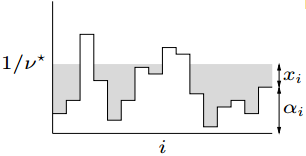
\includegraphics[width=0.4\linewidth]{fig/water-filling.PNG}
\end{figure}
$n$个块,每块高度为$\alpha_i$,用单位水量填充面积,最终的高度为$1/v^\star$
\end{analysis}

\begin{definition}[扰动(perturbed)问题]
\begin{mini*}
    {}{f_0(x)}{}{}
    \addConstraint{f(x)}{\leq u_i}{,\quad i=1,\ldots,m}
    \addConstraint{h_i(x)}{= w_i}{,\quad i=1,\ldots,p}
\end{mini*}
新问题的最优解记为$p^\star(\vu,\vw)$
\end{definition}
\begin{theorem}
若原始问题为凸,则$p^\star(\vu,\vw)$是$(u,w)$的凸函数
\end{theorem}
\begin{theorem}
    设$(\lambda^\star,\vv^\star)$为未被扰动的问题的对偶问题的最优解,则
    \[\forall\vu,\vw:\;p^\star(\vu,\vw)\geq p^\star(0,0)-\vlambda^{\star\T}\vu-\vv^{\star\T}\vw\]
\end{theorem}
\begin{analysis}
    由强对偶性有
    \[\begin{aligned}
        p^\star(0,0)=g(\vlambda^\star,\vv^\star)&\leq f_0(\vx)+\sum_{i=1}^m\lambda_i^\star f_i(\vx)+\sum_{i=1}^p\vv^\star h_i(\vx)\qquad g(\vlambda^\star,\vv^\star)\mbox{定义}\\
        &\leq f_0(\vx)+\vlambda^{\star\T}\vu+\vv^{\star\T}\vw\qquad\vlambda^\star\succeq\vzero
    \end{aligned}\]
\end{analysis}
\begin{theorem}
若原始问题为凸,对偶间隙为0,$p^\star(\vu,\vw)$在$(0,0)$可微,则
\[\lambda_i^\star=-\pd{p^\star(0,0)}{u_i}\qquad\vv_i^\star=-\pd{p^\star(0,0)}{w_i}\]
\end{theorem}

% \begin{analysis}
%     \[\begin{aligned}
%         \vp^\star(\vu,\vw)&=\inf_\vx\lrb{f_0(\vx)\mid f_i(\vx)\leq u_i,h_i(\vx)=w_i}\\
%         &=\inf_\vx S(\vx,\vu,\vw):=f_0(\vx)\\
%         \dom S=\lrb{x\in\dom f_0,f_i(\vx)\leq u_i,h_i(\vx)=\vw_i}
%     \end{aligned}\]
%     需证明$S(\vx,\vu,\vw)$为$(\vx,\vu,\vw)$的凸函数
% \end{analysis}

% 布尔线性规划问题做松弛(relaxation)
% \[x_i\in\{0,1\}\implies 1\geq x_i\geq 0\]